\documentclass[a4paper, oneside]{memoir}% Document class
\usepackage[a4paper]{geometry}			% Margins
\usepackage{lmodern}
\usepackage{graphicx}
\usepackage{pdfpages}
\usepackage{float}
\usepackage{listings}
\usepackage{amsmath}
\usepackage[small,compact]{titlesec}	% No 'chapter' in chapter headings.
\graphicspath{{Media/}}					% Directory that holds images.
\usepackage{hyperref}

\titleformat{\chapter}[hang]
{\normalfont\Large\bfseries}{\thechapter}{1em}{\Large}
\titlespacing{\chapter}{0pt}{*0}{*1}

\titleformat{\chapter}{\Huge\bfseries}{\thechapter}{1em}{}
\titleformat{\section}{\LARGE\bfseries}{\thesection}{1em}{}
\titleformat{\subsection}{\Large\bfseries}{\thesubsection}{1em}{}
\titleformat{\subsubsection}{\normalsize\bfseries}{\thesubsubsection}{1em}{}

\setlength{\parindent}{0pt}
\nonzeroparskip

\newcommand{\figref}[1]{\hyperref[#1]{Figure \ref{#1}}}
\usepackage[disable]{todonotes}					% Todo Notes
\newcommand{\bycykelwithoutspace}{Aalborg Bycykel}
\newcommand{\bycykel}{\bycykelwithoutspace{ }}

\begin{document}
	\thispagestyle{empty} %fjerner sidetal

\hspace*{-1cm}\parbox[b][\textheight][t]{\textwidth}
{

\begin{center}
	\includegraphics[height=5.2cm]{aau-logo-vector}\\
	\vspace{0.25cm}
	%Student Report
\end{center} 

\vspace{1cm}
\begin{center}

\textbf{\Huge {Software 7 - Internet of Things, Bikes}} \\ \vspace{0.5cm}
%\textbf{\Large {Developing Complex Software Systems:}} \\ \vspace{.5cm}
%\textbf{\huge {GIRAF Web Admin and GIRAF Timer}} \\ \vspace{1cm}
\textbf{\Large P7 Project by sw707f14}\\ \vspace{0.5cm}
\textbf{\large 3-9-2014 to 19-12-2014}\\
\end{center}



\vspace{0.25cm}
\begin{center}
\item {\textbf{Participants:}} \\
Dennis Jakobsen\\ Erik Sidelmann Jensen\\ Lasse Vang Gravesen\\ Lars Andersen\\ Mathias Winde Pedersen\\ Søren Skibsted Als\\
\end{center}

\thispagestyle{empty}

\newpage
\thispagestyle{empty}
\mbox{}
}
	\newpage\null\thispagestyle{empty}\newpage
	% Titelbladseksempel til brug på Første studieår.
% Hans Hüttel - hans@cs.aau.dk
% 16. december 2011

% Her begynder selve titelbladet

\thispagestyle{empty}
\begin{titlingpage}
 \begin{nopagebreak}
 {\samepage 
 \begin{tabular}{r}
\parbox{\textwidth}{  \raisebox{-7mm}{\includegraphics[height=4cm]{aau-logo-vector}}
 \hfill \parbox{4.9cm}{\begin{tabular}{l}
{\small Fourth study year} \\
{\small Software} \\
{\small Selma Lagerlöfsvej 300} \\
 \end{tabular}}
}
% \\
\end{tabular}

 \begin{tabular}{cc}
\parbox{7cm}{
\begin{description}

\item[Title:] 

Software 7 - Internet of Things, Bikes
  
\item[Theme:]

Internet of Things


 \end{description}

\parbox{8cm}{

\begin{description}
\item[Project period:]
    P6, spring semester 2014 \\
  \hspace{4cm}
\item[Project group:]
	sw707e14 \\
\hspace{4cm}
\item[Participants:] \mbox{} \\[3mm]
Dennis Jakobsen\\ Erik Sidelmann Jensen\\ Lasse Vang Gravesen\\ Lars Andersen\\ Mathias Winde Pedersen\\ Søren Skibsted Als
   \hspace{2cm}
\item[Supervisor:] \mbox{} \\[3mm]
 Hua Lu \\
\end{description}
}
\begin{description}
 \item[Copies:] 8
 \item[Content Pages:] \pagedifference{startoftoc}{lastpagewithoutappendix}
 \item[Appendix:]  \pagedifference{lastpagewithoutappendix}{LastPage}
 \item[Total Pages:] \pageref{LastPage}
 \item[Completed:] 28-5-2014
\end{description}
 \vfill } &
\parbox{7cm}{
  \vspace{.15cm}
  \begin{tabular}{l}
  \textbf{Abstract:}\bigskip \\
  \fbox{
  	\begin{minipage}{6.5cm}
  	\bigskip
  	{\vfill{\small % Motivation
The bicycle share system in Aalborg is generally subpar compared to other similar systems.
To improve it would provide a better experience for the users.

% Problem statement
Other systems, such as the Gobike in Copenhagen, uses GPS tracking, routing, and other generally useful features. 
To create a website and a supporting system, which allows for tracking, booking, and other such features, would improve the existing system.

% Approach
To resolve this we develop a booking and administration website for \bycykelwithoutspace, and software for simulating stations and bicycles. We made a booking solution for the users of the system, and for the administrators we created pages to provide overview of the system on a whole.

% Results
The website ended up having many features supporting the use and administration of the system.
  	\bigskip}}
  	
  	\end{minipage}
	}
   \end{tabular}}
 \end{tabular}
}
\end{nopagebreak}
\end{titlingpage}

% Her slutter selve titelbladet
	\addtocounter{page}{4}
	\newpage\null\thispagestyle{empty}\newpage
	\thispagestyle{empty}
\section*{Foreword}
\noindent This report was made at Aalborg University in the first semester of the Software Candidate study by the group sw707e14. 
The report was made as a part of the P7 project in the period 3-9-2014 to 19-12-2014. 
We discussed the current system with Aalborg Kommune, whose cooperation was helpful. 
The project was supervised by Hua Lu, whose supervision was much appreciated. \\ \\

\noindent
\vspace{5mm}
\parbox[h]{4cm}{Dennis Jakobsen}\hspace{0.5cm} \makebox[7cm]{\hrulefill} \\ \\
\vspace{5mm}
\parbox[h]{4cm}{Erik Sidelmann Jensen}\hspace{0.5cm} \makebox[7cm]{\hrulefill} \\ \\
\vspace{5mm}
\parbox[h]{4cm}{Lasse Vang Gravesen}\hspace{0.5cm} \makebox[7cm]{\hrulefill} \\ \\
\vspace{5mm}
\parbox[h]{4cm}{Lars Andersen}\hspace{0.5cm} \makebox[7cm]{\hrulefill} \\ \\
\vspace{5mm}
\parbox[h]{4cm}{Mathias Winde Pedersen}\hspace{0.5cm} \makebox[7cm]{\hrulefill} \\ \\
\vspace{5mm}
\parbox[h]{4cm}{Søren Skibsted Als}\hspace{0.5cm} \makebox[7cm]{\hrulefill} \\ \\

\newpage
	\newpage\null\thispagestyle{empty}\newpage
	
	\label{startoftoc}
	\begin{KeepFromToc}
		\tableofcontents
		\newpage\null\thispagestyle{empty}\newpage
		\newpage\null\thispagestyle{empty}\newpage
		\todototoc
		\listoftodos
	\end{KeepFromToc}
	\label{endoftoc}
	
	\chapter{Introduction}
	%disposition:
%politisk mål
	%infrastruktur(letbane, CO2, )
	%sundhed archimedesaaaa
	
%aalborg bycyklen
%problemer
	%ingen statistik og umuligt at finde om der er en cykel uden at gå hen til station
	%ingen sikring om at der er en cykel tilstede
	
%vores løsning

In the current time of Danish politics, a heavy focus has been put on better health \citep{misc:nationalemaalhelbred}.
Additionally, a great focus has been placed on climate change, and how to tackle this \citep{misc:klima}.
A part of a solution to this is getting more people to use bicycles for transportation especially in urban areas.
This limits CO2 pollution due to people not driving in cars and increase health of people due to exercising when bicycling.
A way to make people bicycle more are bicycle sharing systems \citep{misc:impactofbikeshare}, which appear in several cities \citep{misc:cibi, misc:bycyklen, misc:AltaBicycleShare, misc:aalborgbycykelMain}.

The bicycle sharing system that we focus on is Aalborg Bycykel.
It is a system where several bicycle stations are placed around the city of Aalborg, and when you need a bicycle, you travel to one of those stations and retrieve a bicycle.
Then when you are finished using the bicycle you deliver it back to one of the stations.
However, some immediate problems are associated with the currently active system.

One of the problems with the system is that bicycles can easily get lost and there is no way to locate missing bicycles, other than user reports.
Additionally, for a user to know if some bicycle is available, he has to walk to stations until he finds an available bicycle.
Furthermore, if a user wants to be more certain that he can retrieve a bicycle in the near future, there is no way to ensure this other than retrieving a bicycle ahead of time.

These are some of the central issues that is sought to be resolved with the developed system described in the following chapters.
In the developed system, we take other existing bicycle sharing systems into account \citep{misc:cibi, misc:bycyklen, misc:AltaBicycleShare}.
On the basis of this, a booking and status system is developed for the users, and a tracking and statistics system is developed for Aalborg Kommune.
	\chapter{Analysis}
	This chapter includes analysis of the current system already in place in Aalborg, other existing systems, the problem definition, and general requirements.
	\section{Current System}

%Disposition
%kort introduction til hvad det er
%scenarier hvor bycyklen kan bruges
%hvem vedligeholder det
%cyklernes placering
%Positive erfaringer med bycyklen, ref god kilde

\bycykel is a bicycle system where people in Aalborg are able to borrow bicycles to travel around the city.
The system was started in September 2008 as part of the CIVITAS ARCHIMEDES project, which focuses on making bicycles more widely used \citep{misc:aalborgcykling}.
The bicycles can be found in stations located around the city of Aalborg, see \figref{fig:CykelLokationer}.

\begin{figure}
	\centering
	\includegraphics{analysis/CykelLokationer}
	\caption{Bicycle locations \citep{misc:aalborgbycykel}.}
	\label{fig:CykelLokationer}
\end{figure}

As can be seen, the bicycles are mostly located in the center of Aalborg, whereas fewer are placed in other areas.
This means it is easier to borrow and return a bicycle in the central area.

In 2009, 135 bicycles was placed in Aalborg, whereas in 2012 this number had been increased to 200 bicycles \citep{misc:aalborgcykling}.

In order to borrow a bicycle, you need to go to one of the bicycle stations, deposit 20 DKK to unlock the bicycle, then return it to a station when you have no further need of the bicycle \citep{misc:aalborgbycykelregler}, where you will then retrieve your 20 DKK, which makes the system free to use.
This system is built on trust, as if everyone would not return the bicycles to their stations when finished using them, the bicycles would gradually disappear.

\bycykel has had, as of 2012, success with their system. According to a report, if there had not been bicycles more than half of the users would have walked and 5 percent would have driven in a car instead \citep{misc:aalborgcykling}.
Furthermore, it shows that over three season the percentage of bicycles lost has been on maximum 11 percent \citep{misc:aalborgcykling}.

As the bicycles are borrowed by depositing 20 DKK, it means that there is no additional monitoring of where the bicycles are located around the city, other than travelling around the city to locate the bicycles.
This poses the problem that it can be difficult for Aalborg Kommune and the citizens to know which stations have bicycles.
Another problem is if the bicycles are not returned to their stations after use, Aalborg Kommune has difficulty locating such misplaced bicycles.

On their website, it shows that a way for them of locating misplaced bicycles is through citizens reporting lost bicycles by way of SMS and voice mail, or by returning the bicycle themselves claiming the 20 DKK \citep{misc:aalborgbycykelmangler}.
However, if a lost bicycle is not reported or returned by a citizen, the bicycle is practically lost.
The company AFA JCDecaux is in charge of bicycle maintenance and storage during winter time and is also the company in charge of locating the lost bicycles \citep{misc:aalborgcykling}.


These problems could possibly be resolved, and to find inspiration to a solution, other existing systems are analysed hereafter.

	\section{Existing Systems}
A part of analysing and designing a city bicycle system is to investigate the current solutions on the market. 
Therefore an evaluation of existing systems will be conducted.
We found several existing systems implementing different aspects and features of a city bicycle system. 
These systems are listed below:
\begin{itemize}
\item Bycyklen in Copenhagen (gobike)
\item Cibi by AFA JCDecaux
\item Alta Bicycle Share
\end{itemize}
\subsection{Bycyklen in Copenhagen}
The bicycle share system in Copenhagen is called Bycyklen and contains 1,860 bicycles and 100 docking stations \citep{misc:bycyklen}. 
Gobike is a Danish/Dutch company that designed this smart system with a bicycle they call Smart Bike. 
The Smart Bike is equipped with a information screen in the form of a tablet providing the user with an interface to lock the bicycle, select the level of assistance from the electrical system, navigate through the city via GPS and explore new interest points such as cafés and shops.
Furthermore, users of the bicycle system are able to check bus or train arrivals near their current location.
The Smart Bike uses the GPS to send the location, who is travelling, and other statistics about the bicycle such as battery life to Gobike Admin.
Gobike is currently seeing possibilities such as location based marketing, and adjusting the traffic lights according to the cyclist based on the pattern of the bicycle trip and also the weather such as wind speed.
Bycyklen has a very simple 3-step process to rent a bicycle.
\begin{enumerate}
\item Book a Smart Bike ahead from your computer or tablet, find a Smart Bike and log in via the on-board tablet.
\item Unlock the bicycle through the tablet, drive around in the city, possibly assisted by the GPS, paying by the hour.
\item Return the Smart Bike, lock the bicycle and log out of the system via the tablet.
\end{enumerate}
The Smart Bike enables the user to lock the bicycle and securely park it during the bike trip.

\subsection{Cibi By AFA JCDecaux}
The Cibi city bicycle system relies on SMS, where a booking of a bicycle is performed by sending a SMS to a special number with the ID of the bicycle slot in the docking station \citep{misc:cibi}.
The user then receives an acceptance SMS and the bicycle is unlocked or released from the docking station. 
A bicycle trip is charged by the hour, and as with the bike share system in Copenhagen a user can lock the bicycle during the trip. 
This is done through a wire lock which uses a code that the user was given in the SMS when booking the bicycle.

\subsection{Alta Bicycle Share}
Alta Bicycle Share is a company that design, deploys and manages bicycles in USA \citep{misc:AltaBicycleShare}.
The company currently have projects ongoing in nine different cities in USA, with more than thousands stations and over tens of thousands bicycles. 
Alta Bicycle Share believes that humans get the best experience from the environment when the environment is sustainable and enjoyable.
The bicycle stations are design so they can be placed everywhere in the cities without doing any preparation, since they get electricity from solar panels.
Furthermore, the stations are using a cellular connection to upload their data to the main database, so the citizens can see if there are any bikes at a given station.
To rent a bicycle from one of Alta Bicycle Shares system you have to use a card, which can be brought in shops nearby the stations.
These cards then give access to any bicycle for a given time at any station, however, using the bicycle for a longer period of time can lead to a fee.



	\section{Problem Definition}
With the analysis of \bycykel and other similar existing systems performed, it indicates that there is room for improvement.
This leads to the declaration of the problem definition.
It is found that \bycykel is very basic when it comes to technologies, and does not utilise the internet.

In the similar existing systems, GPS, SMS, and card registration is used to locate bicycles.
Furthermore, booking is possible in several of these systems.
This gives inspiration to improvements that can be performed regarding \bycykel, and leads to our hypothesis which is defined as follows.

\begin{center}
\textbf{It is possible to develop a system that makes it easier to use \bycykel, within the context of Internet of Things.}
\end{center}

In order to verify this hypothesis, the following questions have to be answered:

\begin{enumerate}
	\item What are the requirements for a city bicycle booking and positioning system?
	\item How can the booking and positioning system be designed and implemented?
	\item Why should the developed system be used over the currently used system?
\end{enumerate}
	\section{Requirements}
A few criteria have been made, that a system for the Aalborg city bikes should be able to fulfil. In addition to this, the requirements were put into two categories, simple and advanced, and developers should prioritise simple requirements before advanced ones.

Simple:
\begin{itemize}
\item Be able to see how many bikes are available at a given station.
\item Be able to generate data for statistical analysis.
\item Give the possibility of booking a bike, so the user is certain that one is ready at the chosen station.
\end{itemize}

Advanced:
\begin{itemize}
\item Track bikes through fx GPS
\item Predict availability of bikes depending on placement and other variables
\item Use predicted availability to improve booking system.
\end{itemize}
	\section{Target Audience}
The target audience for this project are the regular users of \bycykelwithoutspace, such as tourists and other people in Aalborg that do not have other means of transportation immediately available to them. 
Thus, we strive to develop a system that meets their needs.
In that category goes low-cost and easy access for tourists.
In general we strive to develop the booking part of the system for users who are not particularly tech-savvy, because if the solution works for them, it probably will for most other users as well.

Additionally, the organizations running \bycykel are also part of the target audience, and is kept in mind for the administration part of the system.
	
	\chapter{Suggested Solutions}
	Various suggested extensions for the current system are proposed.
	These solutions are then in turn examined and evaluated, in order to determine if a solution is preferred to others and gives valuable information for the software system.
	An exception to this is the Booking Software examination, which makes a concrete choice on what solution choose.
	\section{Availability of Bicycles}\label{sec:availability}
One of the requirements was that the users of the system need to be able to \textit{see how many bicycles are available at a given station}.
This section covers the suggested solutions for that requirement.
We will look at four different availability checking solutions:

\begin{itemize}
\item Camera based
\item Dock based
\item Chip based
\item WiFi based
\end{itemize} 


% Camera
\subsection{Camera}
A solution with little technological implementation required, would be to use a camera such that users of the system can visually check if any bicycles are available at a given station. 

This solution is good because it is an easy way to add some kind of availability checking without investing in a larger system.

Of course this solution has its downsides, because the information is not reliable in certain situations. 
One example of a situation where a camera would be insufficient would be if it was dark at the station.
You also have to consider that the information transmitted by the camera can be deceiving in that it could show a bicycle that does not really belong at the station and that would make the user come to the conclusion that there are bicycles at the station.
In summary the data is not concise in that it does not provide a standardised way of looking up the information, but rather leaves it up to interpretation for the user.

% Dock
\subsection{Dock}
Another solution that requires a bit more technological implementation is a \textit{Dock} based implementation.
The main idea is that when a bicycle is delivered at a station it is placed in a dock.
A given dock, with some solution that could be a scale or some other type of detector, is then able to register if there is a bicycle located at it.
Each station then contains several docks, and can read from each of them to provide a number for how many bicycles are located at that station. 

%good:
% exact information about how many bikes are available
This solution, unlike the \textit{Camera} solution, provides exact information about how many bicycles are available at a given station with nothing up to interpretation for the user.

%bad:
For this system to work, the bicycles would have to be placed into the docks to provide any correct information.
That is, the system is not registering bicycles misplaced outside the docks.
A potential problem could be if people park their private bicycles in the docks, as this could result in false positives.

% Chip
\subsection{Chip}
A similar solution would be to use chips, such as RFID chips. 
Such a solution is similar in that it provides the same information, namely the amount of bicycles at a given station.
The solution differs, however, in the way this is registered.

One way to do this would be to take inspiration from a car park.
The station would have one or more entrance gateways and one or more exit gateways that are able to read the chip.
When entering the station with a bicycle, the total amount of bicycles will then get incremented, and when leaving with a bicycle it gets decremented.

Another way depending on the distance these chips could be read from, it would be possible to just deposit the bicycles at the station and the station would continually count the amount of bicycles it detects in the near-distance.

% good
These two solutions have in common that they are easy to use, as you come and pick a bicycle and then return it when you are finished.
% bad
On the downside it requires modifying all the bicycles in the fleet, furthermore, if using the car park idea, the stations can end up taking more space than the other solutions. 

% WiFi
\subsection{WiFi}\fxwarning{This doen't work, delete maybe?}
Using WiFi to transmit from the bicycles to the station if it is near, is another solution that could be used.
This solution captures the bicycles located in a perimeter around the station that are on the WiFi network.

This solution provides an estimate of the amount of bicycles available at a given station.
It requires very little in terms of extra infrastructure having to be built.

However, the solution is not as accurate as previously mentioned ones, as bicycles that are already being used but is near the station are registered as well.
Furthermore, it is unclear what costs would be involved with this system and how the bicycles would be powered to maintain the WiFi signal for a longer period of time. 
Maintaining the WiFi signal for a longer period of time when not bicycling may not be necessary as you could assume that when a bicycle is not active, it stays at the same place.
If that is the case, it could be enough to transmit your position when near a station and bicycling, thus powering the WiFi with kinetic energy.

\subsection{Discussion of Solutions}
Among the above mentioned solutions to the problem of determining the availability of a bicycle, a preferred solution has to be chosen. 

The impact of the solutions is measured on the amount of hardware needed to be added to the current system in order to get a working solution. 
For example common to all the solutions requires that a network connection is available at every station because communicating with the system is necessary. 
Furthermore, each solution required different hardware and installations in order to provide the information needed. 

Among the solutions with least impact are \textit{Camera} and \textit{Chip}. 
\textit{Camera} because only an addition of a camera at every station is required. 
\textit{Chip} because only an addition of a non-power-consuming RFID chip would be required.
This is opposed to the \textit{WiFi} solution, which only requires an addition of a WiFi chip, but this chip is power-consuming and therefore requires some kind of additional system to provide power and keeping the bicycles charged.

The \textit{Dock} solution requires an installation of multiple docks at stations, thus not being particularly low impact in terms of required hardware but it does come with some benefits.
Specifically that it is easy for the user to use, and can be more easily extended than other extensions with more functionality such as forced locking.

The \textit{Camera} solution is not considered further because of the possibly inconsistent interpretation by the user, possibly leading to situations where a bicycle is interpreted by a user watching the camera feed to be available, but in fact is not.

The \textit{Chip} solution might be suitable if you only conider the availability of bicycles, however, since there is a requirement for booking of bicycles this solution is not considered further.

The \textit{Dock} solution provides the system with a simple way of determining the number of bicycles docked at each station.
What this solution does not provide is a way of knowing the total number of bicycles currently in the system.
Although a summation of the number of docked bicycles at every station would seem to provide this number, there is an uncertainty that bicycles are stolen or currently in use and not docked in any station.
The \textit{Dock} appears to be the best solution, though it does require some hardware installation.

\subsection{Information Gain}
Various solutions have been discussed, and from a software point of view, we need to know what information each solution can provide.
The \textit{Camera} solution gives access to a camera feed, which is not sufficient, based on the requirement which states you need to provide the amount of bicycles at a station.
The \textit{Dock} and \textit{Chip} solutions gives information regarding how many bicycles are docked at each station, these solutions report this each time the amount of bicycles docked changes.
The \textit{WiFi} solution gives information about how many bicycles are near a given station, and might include bicycles already in use.
The solution can, however, be modified to give the same information as the \textit{Dock} and \textit{Chip} solution, by reporting each time the amount of bicycles in the area changes.

While the \textit{Dock} solution requires installation of the docks at the stations, it does not as such require modification of the bicycles which the \textit{Chip} and \textit{WiFi} do require. 
The \textit{Dock} solution is also very user friendly and easy to use, which is why we think it is the one that fulfils the criteria the best.
	\section{Unlocking of Bicycles}\label{sec:Lock}
There should be a way for the user to unlock a booked bicycle when reaching the station.
This can be solved in several ways, some of these are described hereafter.
We look at several solutions, which are unlock on time, SMS, password based, QR code, and GPS based.

\subsection{Unlock on Time}
This option is independent on whether or not the user is at the station at a specific time.
However, it leads to problems in that a user arriving too early at the station has to wait for the bicycle to unlock, and if the user arrives too late the bicycle might have been taken by another person.
However, this solution is cheap since it only needs the lock on the bicycle, and the communication with the global system, which the other suggestions need as well.

\subsection{SMS}
Whenever the user is ready to retrieve his booked bicycle, he sends an SMS to the system, and the system unlocks his bicycle.
Compared to the previous suggestion, this suggestion does not make the bicycle available to everyone, therefore if the user is late, he can be sure that the bicycle is still available at the station.
Furthermore, if the user comes too early to the station, he is still able to unlock the bicycle and does not have to wait for the bicycle to get unlocked.
Moreover this solution is also cheap since it only needs to have a lock, some kind of receiver for the incoming SMS, and be able to communicate with the global system.
However, this suggestion is not a free solution to the user since they have to pay for the SMS, which can become expensive if the user does not have a Danish mobile subscription.

\subsection{Password}
When the user arrives at the station he has to enter a password at the station to unlock a bicycle.
To be able to do this it requires additional hardware at the station to make it possible to input a password to the system.
Therefore this solution increases the price of each station, as the additional hardware has to be located at every station.
However, it solves the issue that it can become expensive for the user, as this suggestion only costs something for the organisations behind Aalborg Bycykel.

\subsection{QR Code}
In order to unlock a booked bicycle the user has to scan a QR code located next to one of the locked bicycles at the station and navigate to the read link to unlock the bicycle.
This suggestion compared to the previous suggestions does not require any additional hardware and can therefore become cheaper for Aalborg Bycykel.
However, it does require that the user has a mobile device that is able to scan a QR code and send the information over the internet to the system. This could, however, be as expensive for a foreign user as the \textit{SMS} solution due to roaming prices.

\subsection{GPS}
This suggestion uses the GPS of a device to see if the user is close to the station.
If the user is close to the station the booked bicycle gets unlocked.
To use this solution, the user is required to have a mobile device which is able to send GPS information to the system.
This would require that the user has an internet connection as well.
Additionally this is very resource demanding for the mobile device as the use of GPS prevent sleep mode \citep{misc:gpsbatteryusage}, which results in significantly lower battery duration.
Moreover, if the user passes by the station before he actually wants to use the bicycle there is a risk that the station detects this, therefore unlocking the bicycle.

\subsection{Chosen Solution}
The chosen solution should be simple for the user, without requiring specific tools, while still being usable, as specified in \secref{sec:systemCriteria}.

The \textit{Unlock on Time} solution is simple as it does not require anything from the user in terms of equipment, it does, however, have the drawback that the user has to be at the station in time of the unlocking of the bicycle.
It does not leave much flexibility for the user to arrive a little early or a few minutes late.

The \textit{SMS} solution requires that the user has a phone capable of sending an SMS and according to Danmarks Statistik 89\% of people aged 16-74 as of 2013 were able to do so \citep{misc:dstMobilephone}.
It is expected that nearly everyone has a phone capable of sending SMS, but for tourists it might be a problem since not everyone is able to send an SMS to a foreign number or that it might be expensive.
Since the bicycles are also minded towards tourists, this could prove to be a problem.

To be able to use the \textit{QR Code} solution, the user would need some kind of scanner with internet connection, for example a smartphone.
According to Danmarks Statistik, 60\% of the people aged 16-74 in the year 2013 was using internet on their phone \citep{misc:dstMobilephone}.
For the GPS solution, with a smartphone kept in mind, it is important that the smartphone with GPS also has an internet connection to communicate its position to the system, such that the system can react on this.

The \textit{Password} approach covers more users than the other solutions as it does not require people to have a phone, and people can access public internet access points.
The \textit{Password} solution appears to require more hardware installations at the stations, though it does solve the problems of the other solutions in that everyone can use it and the user is in control of when they get the bicycle.
Due to the password based approach covering most users, it is deemed to be the best solution.
In the future, however, the password can also be sent to the user over SMS without additional costs for the user.
	\section{Booking Software}
In order to book a bicycle the user need to interact with some interface.
This interface could be in the form of a website or an application, each with their pros and cons.

\subsection{Website}
The user could make their booking through a website where the user could be asked to create a profile.
The advantage of requiring a user to make a booking could be that the user, as well as Aalborg Kommune, would be able to see statistics about their bicycle usages.
It does, however, have the disadvantage that it is slightly complicated to make the booing, since the user is required to login, although with modern browsers that is able to store usernames and passwords it can make it less complicated.
If the user is not required to create a profile, then in combination with the ideas about unlocking the bicycles, discussed in \secref{sec:remoteLock}, the user would still need to enter some information that can be used to identify him and his booking.
It could be argued that in the long term it would be simpler to create a profile and login, rather than entering the same information for each booking.

\subsection{Application}
The application could be in the form of a mobile application. 
This would simplify the booking process for the users on the move, because the application could be optimised for easy access using touch screen gestures.
The mobile application would exclude people without a smartphone unless both a mobile application and a website are developed.
However, the mobile application could be in the form of a website optimised for phones, and thus allow people to easily use their phone, as well as their desktop computer for booking. 

\subsection{Chosen Solution}
For this project it was decided to focus on only one application.
We decided to focus on a website, since it can be optimised for use on mobiles phones as wells as for desktop computers. 
If the solution had been a dedicated mobile application it would limit the possible users to be people with smartphones, and possibly primarily Danish users because of the roaming prices.
We chose that the better solution was for the user to create a profile in order to book bicycles. 
This would allow Aalborg Kommune to keep better track of who was using the bicycles and the user would not need to enter their user information each time they want to make a booking.
	\section{Tracking Of Bicycles}
In order to counter the loss of bicycles, tracking of the bicycles could be used.
With the tracking, lost bicycles could be located and reinserted into a station.
Furthermore, the tracking can be used for analysis of the bicycling patterns, to see where most bicycles travel to, indicating new hot spots for placing of stations.
Additionally, the tracking can be used to foresee when a bicycle comes to a given station, informing waiting bicycle users of when a new bicycle is ready for use.

Tracking systems which are analysed is GPS and WiFi, and follows hereafter.
\subsection{GPS}
GPS (Global Positioning System) satellites are floating around the earth.
It can be be used to locate the position of a bicycle.
If you equip the bicycle with a retriever it can use the retrieved GPS signals from some of the satellites to estimate the position.
GPS only works when outside, but as you are outside when you bicycle this is not a problem.

The GPS satellites are already floating around the earth, and as of such does not need to be invested in.
For each bicycle it is sufficient to have a GPS retriever to calculate the position, and of course power for it.
Then to report the calculated position, some connection to the developed system would have to exist.
\subsection{WiFi}
Tracking with Wifi is another technique that could be used.
The idea here is to place beacons around the city.
The beacons can then retrieve WiFi signals from a bicycle, and use this to determine the location of the bicycle.

The pro of this type of tracking is that you are not dependent on some externals beacons you do not owen.
On the contrary, you would have to place beacons all around the city of Aalborg in order to precisely locate a bicycle.
Furthermore, you would still need a wifi sender on each bicycle, and as of such you increase the amount of equipment needed to track the bicycles.

\subsection{Chosen Solution}
If tracking of bicycles is implemented, it is found that GPS is the preferred solution, as it can utilise the already existing satellites, and as bicycling is performed outside, the GPS tracking will work most of the time.
	\section{Chosen Solution}
To provide the project with valuable information about how the project could work in the real world, we will also choose a solution for the hardware elements.
This is despite the fact that only the website will actually be developed, along with the API that the hardware will use plus some simulated hardware elements.

For the availability of bicycles, we choose to have docks since it also covers part of the hardware aspect of a different requirement, remote locking.  
For remote locking we also choose to use passwords that need to be input at the station because it is something everyone can do once the booking has been done, as SMS, QR codes, and GPS require phones and might not be suitable for tourists.
If it comes to tracking of bicycles we choose GPS because it requires much less than WiFi to make a reality.

The following provides an overview of the chosen solution using rich pictures.

The server-station relationship is shown in \figref{fig:ServerRichPicture}. 
The server contains collected information from each station, such as bookings, amount of available bicycles at stations, and usage statistics.
It provides booking and amount of available bicycles at stations through a website to the user. 
Usage statistics are provided to the facilitators of the system and gives them the ability to improve it. 

\begin{figure}[h]
\centering
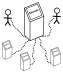
\includegraphics[scale=3]{serverrichpicture/server.pdf}
\caption{The server and the associated stations.}
\label{fig:ServerRichPicture}
\end{figure}

The stations receive the information that allows it to handle bookings done on the server.
They also have the capability of handling booking by themselves, which is then shared with the central server.
Sharing information such as the amount of available bicycles is also something the stations need to be able to do.
The dock that provide the locking/unlocking mechanism along with the bicycle detection ability have to talk to the station, for example when they need to unlock booked bicycle this information needs to be propagated from the server to the station to the individual bicycle.
This can be seen in \figref{fig:StationRichPicture}.

\begin{figure}[h]
\centering
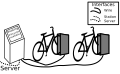
\includegraphics[scale=3]{stationrichpicture/station.pdf}
\caption{The station and the bikes.}
\label{fig:StationRichPicture}
\end{figure}

\begin{comment}
\begin{figure}[h]
\centering
\begin{subfigure}[b]{0.3\textwidth}
\centering

\includegraphics[scale=1]{Bicyclewithlock/bicylewithlock.pdf}
\caption{Locked bicycle.}
\label{fig:BicycleLocked}
\end{subfigure}
~
\begin{subfigure}[b]{0.3\textwidth}
\centering
\includegraphics[scale=1]{Bicyclewithoutlock/bicylewithoutlock.pdf}
\caption{Unlocked bicycle.}
\label{fig:BicycleUnlocked}
\end{subfigure}
\caption{Rich picture of bicycle.}
\label{fig:Bicycles}
\end{figure}
\end{comment}
	
	\chapter{Relevant Material}
	Some background material is needed for the development of a solution and this is examined and discussed.\fxnote{her skal opremses hvad vi skriver om}
	\section{Internet of Things}
This section introduces the \textbf{I}nternet \textbf{o}f \textbf{T}hings (IoT), along with examples of how it is used. 
The section also introduces various hardware considerations to provide the context in which real-world applications for the IoT are developed.

The IoT is the concept describing the interconnection of uniquely identifiable things in the problem domain.
The IoT also includes the virtual representation, the interfaces that allow for manipulation, and information retrieval regarding these things \citep{misc:InternetOfThingsDefinition, misc:InternetOfThingsDefinition2, misc:InternetOfThingsDefinition3}.

Real usage of the IoT manifests as systems to provide some service, either by informing the user about things or allowing an intelligent system to manage those things.
An example of this could be a `smart home' that allows you to use a single device to manage the connected things in your home, such as the lights or the oven in the kitchen \citep{misc:InternetOfThingsExamples}.
One society-wide use for it is the idea of a `smart power grid', where the electricity usage is monitored and managed by an intelligent system that e.g. redirects electricity if a cable has been cut somewhere in the system \citep{misc:smartGrid}.

There are already a lot of things in the IoT, and by 2020 it is estimated that there can be upwards of 26-30 billion things in it \citep{misc:IoTGrowth1,misc:IoTGrowth2}.
This likely requires a shift to the IPv6 protocol as the amount of IP addresses are severely limited by IPv4 \citep{misc:numberOfAddresses} given that the additions to IPv4, such as multiple devices sharing a single IP address, at some point becomes insufficient.

One important aspect of the things connected to the IoT is what technology they use to connect, WiFi or mobile networking are obvious choices of communication means.
For most purposes the connectivity technology has to be low-power and cheap.
Other than WiFi and mobile networking, it is possible to connect things to a server with a cable connecting to the internet, though that is not practical for things that must be mobile.
RFID chips can provide relevant information to an outside observer about the thing itself \citep{misc:rfid} with active research in making it low-cost and low-power \citep{misc:rfid2}.

The geographical location in the IoT matters, especially for sensors where the location provides important context for the accessed information \citep{misc:locationMatters}.
For example if there is a station for bicycles in a bicycle sharing system that needs to provide information regarding the amount of bicycles at the station, it is important for the usage of the information that it also provides the actual location of the station, if that is not otherwise known.

In order to give more detail on IoT, aspects about identification, communication, and software is given.

\subsection{Identification}
In order to uniquely identify the things in the IoT, different approaches can be taken.

One idea is to use the IP address of an object, which has relation to the previously discussed IPv4 versus IPv6 issue.
With IPv6, this approach would have enough addresses to uniquely identify a large number of things.
Given IPv6 has a theoretical possibility of $3.4 \cdot 10^{38}$ unique addresses \citep{misc:ipv6}, not having enough addresses would not be a problem in the foreseeable future.

When you have a unique address, you can use that to uniquely identify the given thing.
An example of use is the power grid, where each power station can uniquely be identified with the IPv6 address, and as such, in case of malfunction in one of the grid connections, it would be possible to identify the stations lacking power.

\subsection{Communication}
In order for the IoT to work, it is necessary to have a communication established.
If that was not the case, the things would not be part of the IoT, as the central idea is that you can communicate over the internet.

One idea of communication for sensors is as follows.
Each sensor has access to the internet to contact a web service with their given reading.
However, it is unrealistic that each sensor alone is directly connected to the internet, and as such, other alternatives can be performed.
One such alternative is that a thing consists of a communication device connected to several sensors and the internet.
The communication device can then read from the sensors and contact the web service.

However, the communication does not end at this point.
The idea is that the communication is not limited to machine-machine communication, but is expanded to communication over the internet, such that the things of the IoT can be contacted from anywhere on the internet.

\subsection{Software}
Examples of Software that utilise the IoT are given to get a concrete idea of the power of the IoT.

We expand on the example of the smart power grid.
Such a power grid uses the information it has about each section of the grid, to ensure that there is sufficient power reaching every part of the grid, even in cases where part of the grid malfunctions.
This ability is achieved through the system being able to automatically reroute the power flow in the grid, so power flows through functioning areas to reach the parts that would otherwise have been affected by the malfunction.

Another example is the mentioned home automation system.
For such a system, the things of the house being the lock, coffee machine, lights, washing machine etc, is then the central parts.
If the things of the house is connected to the IoT, it is possible to connect to those devices and control them over the internet.
This has several advantages, which includes ensuring the door is locked, preparing coffee before you get home, and other actions you may want to do with the things of your house, even though you are at work or on vacation.
	\section{ER-Diagram}
In order to have an idea of how the database for handling bookings and location of bicycles and their relation to the location of the stations, an ER-Diagram was made, see \figref{fig:er-dia}.

\begin{figure}
	\centering
	\includegraphics[scale=0.4]{relevantmaterial/erdiagram}
	\caption{ER-Diagram for database overview.}\label{fig:er-dia}
\end{figure}

As seen in the diagram, the entities consists of bicycle, dock, station, booking, and account.
An account consists of a username and email, which both must be unique, and a phone-number and password.
These attributes are common for an account entity, with the phone-number being special in that the idea is they will receive the booking-password over SMS.

In relation to this is the booking entity, where it can be seen that a user can have zero to many bookings whereas a booking is registered to one and only one account.
The booking then has a booking-id, to uniquely identify a booking, a start-time, such that a station knows when to lock a bicycle, and a booking-password used to unlock a bicycle at the given start-time if a correct password is entered.
The idea is that if a booking is not used in a given timeframe at the start-time, the booking will be removed, to prevent spamming of bookings without use.

A booking is also tied to a station, such that a booking is located at one and only one station, whereas a station has zero to many bookings.

A station has the attribute station-id, to uniquely identify the station.
Furthermore, it has a name, which is thought to be used to give a meaningful description of a given station.
We are aware that the name could be used as a primary key, but having an id as the primary key unlocks the possibility of duplicate names, which might be desired for stations located at different spots in the city, example could be two stations named "AAU Bycykel Station" which is a quite generic name.

In addition to this, a station has a location, which is used to easily place a station on a map, and can also be used for calculations such as distance between a given station and bicycle.
A station also has two derived attributes, which are available-bicycles and amount-of-bookings, these are attributes that is beneficial to show to the user, such that they can see if it is possible to gather a bicycle at a given station.

Next is the dock entity, which is a weak entity, as it cannot exist without a station.
This represent the real-life situation with stations located around the city, and each of these has a number of docks.
The dock only has one attribute, which is the dock-id, used to identify a dock in combination with a station-id.

The interesting part of a dock is its relation with a bicycle.
A dock may or may not hold a bicycle, which is represented with the holds relation.

The bicycle entity then consists of a bicycle-id, to uniquely identify a given bicycle, and a location, which can be used to locate the given bicycle, as can be beneficial to calculate distances, but also to locate lost bicycles.
	\section{Model View Controller}\label{sec:mvc}
The Model View Controller (MVC) is a design pattern widely used in programming to separate the program into different layers called `Model', `View', and `Controller'.
This provides the advantage that the structure gains clarity and becomes easier to maintain as it separates responsibility to individual layers, and is why this design pattern is used.

An illustration of MVC can be seen in \figref{fig:MVC}.
\begin{figure}[h]
	\centering
	\includegraphics[scale=0.6]{relevantmaterial/MVC}
	\caption{Illustration of the MVC pattern.}\label{fig:MVC}
\end{figure}

The `Model' layer provides abstraction over the data stored in the database.
Additionally it provides business logic to work on this data and functions to modify the state of the database.

A request from the browser is interpreted into a controller action.
The `Controller' provides a set of 'actions' that can be executed based on the interpretation of the browser request. 
These actions then use functions in the `Model' layer and uses views to show an representation of the model, e.g. a table or a map of stations. 
These views are then presented to the user through the browser.
A controller may include multiple views to get a HTML page generated for the client to view.
As multiple views may be included by the controller, it may use separate views for the header, the body, and finally one for the footer. 
These multiple views allow for reuse of views and is also well suited for asynchronous loading of smaller parts of a page.

It is important to note that there is a single model layer, consisting of multiple entities (e.g bicycle and booking) and their associated services.
Additionally, it is a good practice to have multiple controllers, which each handle different parts of the website.
An example is to have a home and user controller.
With the user controller taking care of everything connected to user login, editing of profile, logout etc. and some actions could be moved to a separate controller if it becomes unmanageable.
The home controller takes care of the presentation of the frontpage.
To ensure better code clarity, the controllers are split into different responsibility areas of the website, each such controller containing a set of actions related to its responsibility area.

In addition to the better code clarity, as the website is organised in the way it is, working with the same model, the layout of the website can easily be changed, by including other views or developing additional controllers for other work routines.
This is related to the high modularity you gain with the MVC pattern, leading to high cohesion (elements in a module belong together to a high degree) and low coupling (low interdependence between modules).

However, some things need to be loaded asynchronously for increased usability, which is where AJAX comes in.
	\section{Asynchronous JavaScript and XML}
Asynchronous JavaScript and XML (AJAX) is a way to create a website update parts of the website without user interaction.
By using AJAX parts of the websites can be updated without reloading the whole website every time, which makes the use of a website much more smooth.
Even though XML is a part of the AJAX name, it is no necessary to use when using AJAX, other methods to send the data can be used, an example could be to use JSON.
When using JSON, data is encoding where after it is printed on a asynchronous website, which the website then decode and reload the part that it effects.

The reason to use AJAX is to improve the usability of a website, as well as the performance of a page.
An example of this is e.g. when rating a film on www.IMDB.com then when pressing the rate, the website does not reload, but register and call the database that an update have occurred. \fxnote{kilde her}
The AJAX should be used whenever the user makes an interaction that does not need to do anything to the website, but only update information on the database, this could be changing the password of a user. 
Furthermore, AJAX should be used when updating only a part of the website, so that the website should not be refreshed before updating this part of the website.
	
	
	\chapter{Architecture}
	Meta-language for the architecture
	
	\chapter{Behaviour}
	This chapter will outline the behaviour of the system in the situations listed in \secref{sec:behaviourProblems}.
	\section{Scenarios}\label{sec:behaviourProblems}
In this section we will raise some questions that need attention or describe a situation where a behaviour needs to be defined for the system.

\textbf{Questions}
\begin{itemize}
\item When should a bicycle become unavailable for others, as a result of a booking?
\item When should a bicycle become available again after a booking has exceeded its reservation time?
\item How often does the GPS needs to read data?
\end{itemize}

\begin{description}[style=nextline]
\item[Problem 1.1] Consider the scenario where a user $u_1$ makes a booking $b_1$ on the website at time $t_1$ wanting to reserve a bicycle for time $t_3$. Before time $t_1$ another user $u_2$ made a booking $b_2$ of a bicycle for time $t_2$. Both users made a booking at the same station, and the amount of available bicycles for that station was for both users 1. Under the assumption that a bicycle cannot be locked and thereby reserved before some amount of time, say $t_{before}$, before usage, this scenario is possible in the following way.

First consider this definition of a time $t$, it is a time represented as the number of seconds from Thursday, 1 January 1970 at 00:00:00 UTC, which is the Epoch time, as of such comparisons such as $>$ is just computed as usual on numbers.
Let, 
$$TSB(b) = \{(t_1,t_2) \;| \;t_1 = st(b) - t_{before} \land t_2 = st(b) \land t_1 \leq t_2 \}$$
where,
\begin{itemize}[align = left]
	\item[$st(b)$] is defined as the start time of booking $b$.
	\item[$TSB(b)$] defines the Time Span Before of booking $b$.
\end{itemize} 

\begin{figure}[h]
	\centering
	\includegraphics[trim = 1cm 19.7cm 0cm 0cm,clip]{behaviour/booking-illustration}
	\caption{Booking scenario illustration.}\label{fig:booking-illustartion}
\end{figure}
Then the scenario is given if $TSB(b_2)$ starts before $TSB(b_1)$ and $TSB(b_2)$ starts after $t_1$, we have a situation as can be seen in \figref{fig:booking-illustartion}.
As can be examined from the illustration, a problem occurs, under the assumption that no new bicycles gets delivered or taken from the given station in the given time-line, and where the amount of available bicycles before the lock-time of $b_2$ is 1.

The problem for user $u_1$ is then at time $t_1$ it appeared that a bicycle was available, but the bicycle will be locked for user $u_2$ (although not entirely certain, see Problem 1.2) before it will be locked for $u_1$ resulting in an availability count of 0 for $u_1$, thereby having no bicycle to lock for $u_1$.

\item[Problem 1.2] Having a booking system that is capable of capturing the state of each station, giving available bicycles and available free docks, along with the ability to borrow a bicycle without interacting with the booking system, imposes an element of unpredictability.

Given the scenario where a user reads the state of a station and makes a booking $b$ on that station at a time $t$ starting before $TSB(b)$, no certainty is provided that ensures that a bicycle is available to lock in $TSB(b)$. 
This is due to other users, who might have borrowed the rest of the bicycles at that station before $TSB(b)$, thus preventing the station from locking the desired amount of bicycles.

\fxwarning{Forstår det ikke, fungerer systemet sådan som det antager? Falder antal tilgængelig cykler ikke når man laver en booking?}
\item[Problem 1.3]
For how often a GPS have to read, some information have to be described before hand.
First it is necessary to decide what kind of information is desired from the GPS.
If the desired information is just current position of the bicycles, infrequent updates work just as well as frequent ones, however, if information about bicycle routes are what is desired, then more frequent updates would be necessary.

To illustrate this we can look at \figref{fig:gpsCircles}, the green circle in this picture is where the bicycle is at the last update, where the rings indicate where you can be after some seconds.
To look at time intervals the information of how often a GPS can reed have to be determined, this is determined by looking at datasheets of GPS, here a datasheet \citep{manual:gpsDataSheet} states that the GPS can read 50 times per second, therefore anything higher than that can be chosen.
In the figure the three circles represent 10 (blue), 30  (yellow), and 60 (red) seconds time intervals at a speed of 20 km/h.
The overlay on the map represents the distance that can be covered if travelling in a straight line, however, when travelling with a bicycle straight line travelling is not very common.
20 km/h was chosen as the speed because this is the average speed of bicycles where all the intersection lights are green \citep{misc:bicycleStatistics}.

We have chosen to let the GPS update at least every 30 second, since this makes it possible for us to determine the precise route of the bicycle.
The reason why 30 seconds was chosen is because you are not able to move that far in 10 seconds, however, when tracking only every 60 second it is possible to take alternative routes than the shortest route.


\begin{figure}
	\centering
	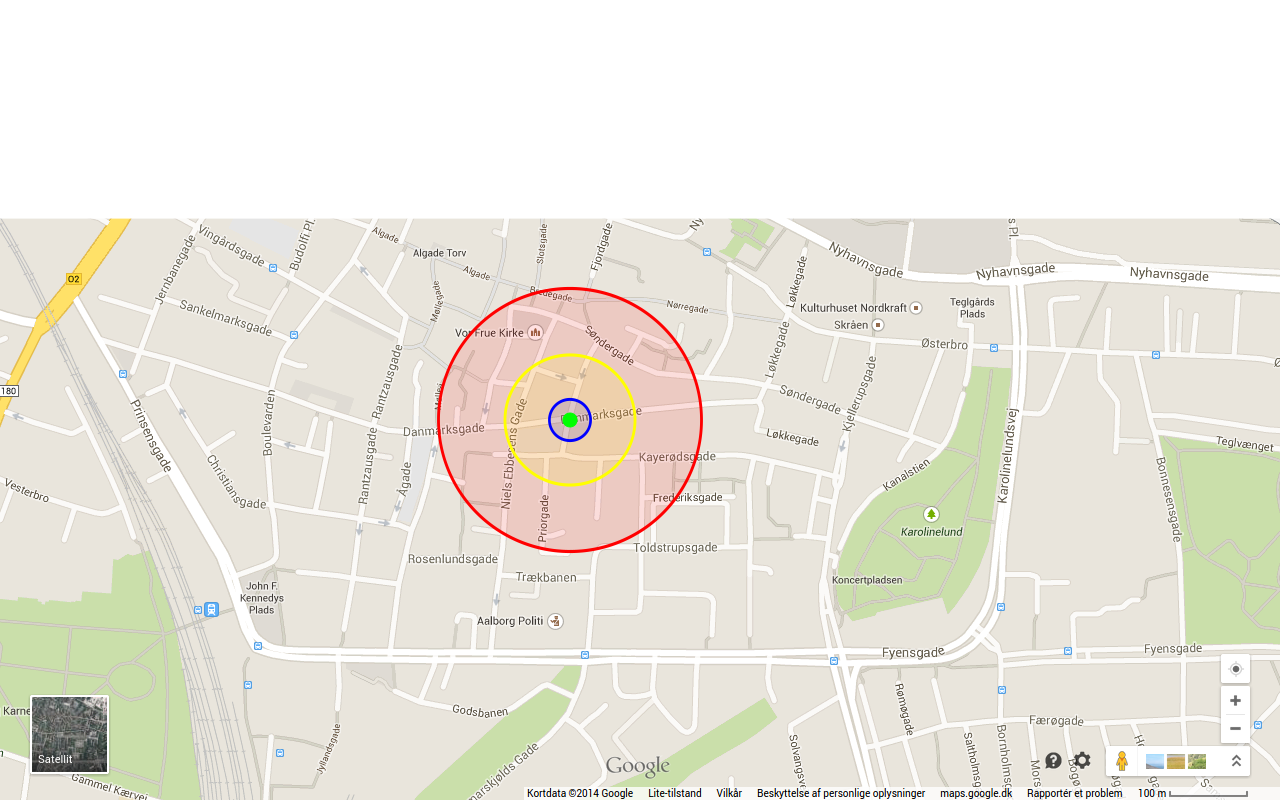
\includegraphics[scale=1]{GPScircles}
	\caption{Distance coverage with 20 km/h.}
	\label{fig:gpsCircles}
\end{figure}
\end{description}


		
	\chapter{Prototypes}
	This chapter will present prototypes of the visual design for system.
	\section{Prototype}
In order to get a better idea of how the website should look like, various prototypes were drawn.
As they are prototypes, they are by no means a representation of the final product, but more of a source of inspiration and brainstorming, to consider when developing the website.
Throughout this section, one prototype sketch for each part of the website considered with prototyping, is presented, explained and discussed.

\begin{figure}[h]
	\centering
	\includegraphics[scale=0.6]{design/prototype-about}
	\caption{About page.}\label{fig:prototype-about}
\end{figure}

First, we take a look at \figref{fig:prototype-about}.
This illustration presents a draft of the about page, it is structured as a standard about page with some description of the organisation behind the website as well as a pretty picture to look at.
What is more interesting to see in this illustration is the first draft of the menu bar.
The menu bar consists of links to about, status, book, and login links, each of which has their page(s) illustrated hereafter.


\begin{figure}[h]
	\centering
	\includegraphics[scale=0.6]{design/prototype-status}
	\caption{Status page.}\label{fig:prototype-status}
\end{figure}

\begin{figure}[h]
	\centering
	\includegraphics[scale=0.6]{design/prototype-booking}
	\caption{Booking page.}\label{fig:prototype-book}
\end{figure}

\begin{figure}[h]
	\centering
	\includegraphics[scale=0.6]{design/prototype-about}
	\caption{Booking history page.}\label{fig:prototype-book-history}
\end{figure}

\begin{figure}[h]
	\centering
	\includegraphics[scale=0.6]{design/prototype-user}
	\caption{User pages.}\label{fig:prototype-user-overall}
\end{figure}

\begin{figure}[h]
	\centering
	\includegraphics[scale=0.6]{design/prototype-edit-user}
	\caption{Edit user page.}\label{fig:prototype-edit-user}
\end{figure}

	
	\chapter{Implementation}
	This chapter covers implementation details.
	
	\section{Framework}
To set up the Model-View-Controller architecture for development, a modified PHP MVC framework is used, see \citep{misc:mvc-framework} for details on it.

The framework provides a controller base class that the new controllers inherit from, mainly providing a database instance.
It also provides an application class that handles URL parsing and navigation to the correct pages based on the URL.
The framework also provides a directory structure. 
You can, for example, add a controller to the controller directory and the Application class is able to load them. 
Another example is to add a model to the model directory and that can be used by the controllers. 
Additionally, you can add views to the view directory and they can be included by the controllers.

Some modifications are applied, in that instead of a single model class per entity in the database, it is split into an entity class, wrapping the database data, and an associated service, implementing CRUD behaviour to work on said entities in the database.
This is useful, as it separates the data and the methods working on the data, as it improves cohesion and reduces coupling in the code.
We also change class loading to use autoloading instead. This is to not be enforced to include all files manually.
	\section{Interfaces}\label{sec:interfaces}
As is described in the design, some communication between the stations and the database has to be established, to retrieve bookings etc.
This communication is established through the three interfaces gpsregister, websitetostationnotifier and stationtodbregister.
These interfaces being from website to station, station to database, and bicycle to database.
Each of these interfaces are described below.

\subsection{Website to Station}\label{sec:webToStationI}
This section is about the websitetostationnotifier interface from \figref{fig:overallarch}.
The website has to establish contact to a station when a booking or un-booking has been performed.
It is evident that this is important, as the stations need to be notified to keep track of bookings involving themselves as station.

This contact is established through TCP/IP, and is used in implemented notification methods.
These being \texttt{notifyStationDockChanged}, \texttt{notifyStationBooking} and \texttt{notifyStationUnbooking}.
The call to the notification methods is added in the \textit{BookingService}, as each time a booking is created, updated, or deleted, it is called through BookingService, and as of such we ensure the notification method is always called.

In general, the notification methods work in the following way:
\begin{itemize}
	\item Construct JSON encoded message to be sent to the station.
	\item Create the TCP socket.
	\item Connect the socket to the station involved with the booking.
	\item Send the data to the station.
	\item Close the socket.
\end{itemize}

The reason the message is JSON encoded, is to have a standard way of encoding data, which can be easily decoded by the station.
It is then up to the station to parse this information and perform the action specified in the message.
How the JSON encoded message looks like, as well as how the station handles this notification is elaborated in \secref{subsubsec:listener}.

\subsection{Station to Database}
This section is about the stationtodbregister interface from \figref{fig:overallarch}.
The station to database interface is important in order to register when a bicycle has been taken at a station or returned to a station, in order to give correct information on the website status page.
Additionally the interface is used to retrieve information about bookings registered in the large database, in case of power-up of a station.

The interface has been implemented in a SOAP encoding by help of the NuSOAP library.\fxwarning{kilde her}
This library makes you able to write regular PHP functions and then register these with the NuSOAP library, in order to have a webservice generated.
Bear in mind that all methods registered with NuSOAP needs to have a return value and as such a dummy boolean value is used where no other return value is needed.

An example of the implementation of an update and read operation on the database is presented in \lstref{lst:bicycledockstationreturned}.

\begin{minipage}{\textwidth}
\begin{lstlisting}[caption = {Method for registering a bicycle as been returned to a dock at a given station.}, label = {lst:bicycledockstationreturned}]
$server->register('BicycleReturnedToDockAtStation',
	array('bicycle_id' => 'xsd:int',
	'station_id' => 'xsd:int',
	'dock_id'    => 'xsd:int'),
	array('return' => 'xsd:boolean'),
	$SERVICE_NAMESPACE,
	$SERVICE_NAMESPACE . '#soapaction',
	'rpc',
	'literal',
	'Registers that a given bicycle has arrived at a given dock at a given station'
);
function BicycleReturnedToDockAtStation($bicycle_id, $station_id, $dock_id)
{
	global $db;
	$stmt = $db->prepare("UPDATE dock SET holds_bicycle = ? WHERE station_id = ? AND dock_id = ?");
	$stmt->bind_param("iii", $bicycle_id, $station_id, $dock_id);
	$stmt->execute();
	$stmt->close();
	
	[...]
	return true;
}
\end{lstlisting}
\end{minipage}

If you take a look at \lstref{lst:bicycledockstationreturned}, the code is split into two parts, line 1-11 and line 12-21, which handles different parts of providing a method to register that a bicycle has returned to a dock at a given station.

Line 1-11 takes care of registering the PHP function, such that it can be included in the auto-generation of the SOAP encoded webservice.
As can be seen from this specification, we tell the NuSOAP library the name of the function to register on line 1.
Then line 2-4 specifies the input parameters, line 5 specifies the return value, and line 6-11 is less interesting parts which deals with how the method should be represented in SOAP.

Line 12-21 is the actual method for registering that a bicycle has been return to a dock at a given station.
This is performed with use of prepared statements, as can be seen in line 15-18, which is done to prevent SQL injection.
As you can see, the actual statement expresses an update on the dock, such that the dock, where the bicycle has been placed, gets a reference to that bicycle.

\begin{minipage}{\textwidth}
\begin{lstlisting}[caption = {Method for reading all bookings for a given station}, label = {lst:getallbookingstation}]
$server->register(
	'GetAllBookingsForStation',
	array('station_id' => 'xsd:int'),
	array('return' => 'tns:BookingObjectArray'),
	$SERVICE_NAMESPACE,
	$SERVICE_NAMESPACE . '#soapaction',
	'rpc',
	'encoded',
	'Get all bookings for station'
);
//in case you want to read everything.
function GetAllBookingsForStation($station_id)
{
	//returns all bookings from database from a given station, as a json encoded array.
}
\end{lstlisting}
\end{minipage}

An example of a method that reads from the database is the \textit{GetAllBookingsForStation} function, seen in \lstref{lst:getallbookingstation}.
Such a method is for example useful when first booting a station where its local database is empty or that the local database data is outdated, e.g. it has been offline for some time.

Taking a look at line 1-10, you see the registration of the PHP function for integration in the SOAP specification.
As can be seen, it utilised a custom type called \textit{BookingObjectArray}, which is an array type used to contain multiple JSON encoded strings that represents bookings.
The result is a JSON encoded array and can be used by the given station to traverse the array returned and decode each string to get its corresponding booking information.

\subsection{Bicycle to Database}
% Ting der skal skrives om:
% - Caching på cykler, dårlig dækning, data skal ikke gå tabt
% - Hvor ofte skal der sendes data
% - Alternativer til f.eks. GSM moduler?
\fxwarning{Se comments i source her.}
This section is about the gpsregister interface from \figref{fig:overallarch}.
The interface from bicycle to database, is an interface that is needed to register the location of a bicycle, as GPS tracking is decided to be implemented, due to the meeting held with Aalborg Kommune.
The idea is that each bicycle use the interface to inform the system where it is located, according to the coordinates received from GPS.

The interface is implemented in the same fashion as the interface from station to database.
As such, it is implemented as a SOAP web-service, using the NuSOAP library to gain the an encoding that makes the interface easy to call.
There exists one method, the \textit{RegisterGPS} method, which takes three arguments, the bicycle-id, latitude, and longitude.
The way this interface is constructed is similar to the other SOAP encoded interface, but where the bicycle location is updated instead.
	\section{Model \& Model Services}
This section will describe the model and model service layer.
It will illustrate this by giving an example model, showing what they it looks like and what it does and then illustrating the corresponding service.
It will then provide an overview over the rest of the models, their model services and their functions.
For more detail about Model-View-Controller architecture, see \secref{sec:mvc}.

The Bicycle model can be seen in \lstref{lst:bicycleModel}. Our modification to the original MVC skeleton here is then that instead of using the models to implement behaviour, we use it to model the corresponding database table.

\begin{minipage}{\textwidth}
\begin{lstlisting}[language=php, label=lst:bicycleModel, caption={Bicycle Class}]
<?php
class Bicycle
{
    public $bicycle_id = null;
    public $longitude = null;
    public $latitude = null;

    function __construct($bicycle_id, $latitude, $longitude){
        $this->bicycle_id = $bicycle_id;
        $this->longitude = $longitude;
        $this->latitude = $latitude;
    }
}

?>
\end{lstlisting}
\end{minipage}

The corresponding BicycleService, though very truncated, can be seen in \lstref{lst:bicycleService}. The BicycleService implements CRUD methods for the Bicycle model.

\begin{lstlisting}[language=php, label=lst:bicycleService, caption={BicycleService Class}]
<?php

//create read update delete
class BicycleService implements iService
{
    private $db = null;

    function __construct($database){
        try{
            $this->db = $database;
        }
        catch(Exception $ex){
            exit("Unable to connect to database " . $ex);
        }
    }

    /**
     * Function that creates a new bicycle
     * @return the created object
     */
    public function create($bicycle)
    {
        if(validate($bicycle))
        {
            $stmt = $this->db->prepare("INSERT INTO bicycle(longitude, latitude) VALUES (?,?)");
            $stmt->bind_param("dd", $bicycle->longitude, $bicycle->latitude);
            $stmt->execute();
            $id = $this->db->insert_id;
            $stmt->close();
            return new Bicycle($id, null, null);
        }
        else
        {
            return null;
        }
    }
    
    //[...]
}

?>
\end{lstlisting}

The models and their associated services, are as follows:

\begin{itemize}
\item Account \& AccountService -- Account for the database representation, and AccountService for CRUD functionality and verifying logins.
\item Bicycle \& BicycleService -- Bicycle for representation and BicycleService for CRUD.
\item Booking \& BookingService -- Booking for representation and BookingService for CRUD and getting/deleting bookings for a specific user.
\item Dock \& DockService -- Dock for representation and DockService for CRUD and determining if a dock is currently holding a bicycle or getting all docks at a station.
\item Station \& StationService -- Station for representation and DockService for CRUD and special functionality such as getting counts of available bicycles at stations or for searching for a station.
\end{itemize}

We also provide various helper functionality in Tools and ViewHelper. 
In Tools we provide helper functionality for determining if the user is logged in, for including CSS and JavaScript, and for validating special fields like email addresses.
In ViewHelper we provide helper functionality for printing error or success messages, and printing date components.

 The next section will show how they are used in the context of the controller layer.
	\section{Controller}
This section will show how the controller layer works. 
It will illustrate this by giving an example controller, showing what it looks like and what it does.
It will then provide an overview of the rest of the controllers and their function.
For more detail about Model-View-Controller architecture, see \secref{sec:mvc}.

In \lstref{lst:homeController}, part of the Home Controller can be seen. 
It defines an `action', this action is what is pointed to by the client. 
For space saving purposes all actions but the index action have been removed.
It then uses two services, StationService and BookingService. 
The StationService is used to retrieve an array of all stations(lines 8--9), and the BookingService is used to retrieve an array of all active bookings for the currently logged in user(lines 11-14). 
This illustrates the general idea behind the separation of the entities(The Models) and the services corresponding to those models.
It then uses the information loaded by 'including' views, and these views then use the information for displaying.

\begin{lstlisting}[language=php, label=lst:homeController, caption={Home Controller Class}]
<?php
class Home extends Controller
{
    public function index()
    {
        $this->title = "Home";
        $currentPage = substr($_SERVER["REQUEST_URI"], 1);
        $stationService = new StationService($this->db);
        $stations = $stationService->readAllStations();

        if (Tools::isLoggedIn()) {
            $bookingService = new BookingService($this->db);
            $activeBookings = $bookingService->getActiveBookings($_SESSION["login_user"]);
        }

        require 'application/views/_templates/header.php';
        require 'application/views/home/index.php';
        require 'application/views/_templates/footer.php';
    }
    // [...]
}
\end{lstlisting}

The controllers and their `actions' are as such,

\begin{itemize}
\item Home {\begin{itemize} 
            \item Index -- The homepage and what is shown by default.
            \item Unbook -- For unbooking a booking for the logged in user.
            \item Book -- For booking a booking for the logged in user.
            \end{itemize}}
\item User {\begin{itemize} 
            \item Index -- Nothing special.
            \item Logout -- For logging out.
            \itme Login -- For logging in.
            \item createUser -- For creating a nw user.
            \item changePassword -- For changingthe password of the logged in user.
            \item editProfile and changeAccountInfo -- For changing email or phone number of the logged in user.
            \item forgotPassword, forgotPasswordForm, resetPassword, and resetPasswordForm -- For resetting a lost password.
            \end{itemize}}
\item About {\begin{itemize} 
            \item Index -- Showing an about page.
            \end{itemize}}
\item Admin {\begin{itemize} 
            \item Index -- Showing a special map for administrative purposes.
            \end{itemize}}
\item Ajax {\begin{itemize} 
            \item Index -- Does nothing.
            \item getBicyclePositions -- Get a JSON encoded array of coordinates of all bicycles that have not null coordinates.
            \item getStations -- Get JSON encoded information about stations for dynamic updating.
            \item getFreeDocksList -- Get json encoded information about amount of free docks at all station.
            \end{itemize}}
\end{itemize}

What views look like will be illustrated in the next section.
	\section{Views}
This section describes the view layer and what it does, illustrating by example.

In \lstref{lst:homeIndexView} a truncated version of the home index view can be seen. 
Most of it is normal HTML, but the important part is how it utilizes variables set in the controller, because a view is included by a controller, it gives access to the variables of the controller. 
This allows it to use them to generate more HTML as can be seen lines 6-10 where it uses the array of stations set in the controller to output option elements in a select element.
It can also use defined methods, as shown in line 13-19.

\begin{lstlisting}[language=html, label=lst:homeIndexView, caption={Home Index View}]
[...]
<form action="/Home/Book/" method="post">
    [...]
    <select name="station" id="stations" style="width: 243px;" onchange="UpdateMarker()">
    <option value="0" disabled selected>- Select Station -</option>
    <?php
    foreach($stations as $station){
        echo '<option value="'.$station->station_id.'">'.$station->name.'</option>';
    }
    ?>
    </select><br />
    [...]
    <?php
        if (Tools::isLoggedIn()){
            echo '<input type="submit" value="Book" />';
        } else {
            echo '<a href="/User/Login/">Login</a>';
        }
    ?>
    [...]
</form>
[...]
\end{lstlisting}

	\section{Google Maps API}\label{sec:googlemapsapi}
The Google Maps API \citep{misc:googlemapsapi} is used to show the map on both the front page and the admin page.
However, both of these pages use the API differently, the front page uses the API to show the map with the stations that are currently in the system, whereas the admin page visualises where all the bicycles are located.

To use the API, the construction of the map is done first, which can be seen in \lstref{lst:mapoptions}.
Map options are chosen here, these options are e.g. the center of the map, which zoom level the map should have, and the style of the map.

\begin{minipage}{\textwidth}
\begin{lstlisting}[caption={Construction of the map}, label={lst:mapoptions}, language=Javascript]
var mapOptions = {
	zoom: 13,
	center: aalborg,
	panControl: false,
    zoomControlOptions: {
		style: google.maps.ZoomControlStyle.LARGE,
		position: google.maps.ControlPosition.RIGHT_TOP,
	}
};
\end{lstlisting}
\end{minipage}

After the map is constructed the map is filled with either the stations or the bicycles, depending on the page.

For the front page the stations are inserted into the map by use of AJAX.
For each station, the work-flow of this is as follows:

\begin{description}[style=nextline]
	\item[Gather data]
	Use the stationservice to read data to be displayed on map.
	\item[Create info window]
	The info window is a window that appears whenever the user clicks on a station marker.
	The info window shows information about the station, which is the name, amount of free bicycles, and the amount of free docks.
	\item[Marker creation]
	Create a marker, which are the bulletpoints indicating the station on the map.
	The creation of the marker contains position, title, icon.
	\item[Assign listeners]
	Assign listeners to the marker clicks, in order to show the infowindow for the given marker when the marker is clicked.
\end{description}

\begin{figure}[h]
	\centering
	\includegraphics[scale=0.7]{googlemarkermap}
	\caption{Google map with station markers and info window shown}
	\label{fig:googlemapmarkerinfowindow}
\end{figure}

An example of the final google map with markers placed can be seen in \figref{fig:googlemapmarkerinfowindow}.

For the admin page the markers are bicycles, which are updated at a set frequency using AJAX, and is created in a similar fashion, just by other objects placed on the map.
The main purpose of the admin tracking page is to be able to see where the different bicycles are at a given time, which is the reason why the markers are updated once in a while.
For the purpose of this project it updates every tenth second, to be able to simulate how it could look like, however, in the real system every tenth second might be too often, depending on how often the GPS's of the bicycle send data to the database.
For the update of the marker position AJAX is used to get all the positions of the different bicycles, which allows the makers to move without refreshing the page.
	%!TEX root = ../../main.tex
\section{Station Software}
The station software package contains two aspects, software intended to be run on the stations, and software to simulate the hardware we do not have access to, used as proof of concept.
For an overview of the station structure, see \figref{fig:stationarch}. 
However, to use these two aspects a GUI is needed, and is described hereafter.

\subsection{GUI}
The Main GUI window has two parts, which can be seen in \figref{fig:stationMain}, part one is the station software, and part two is for the hardware simulation, which is explained later in this section.

\begin{figure}[h]
	\centering
	\includegraphics[scale=0.4]{stationsoftware/mainwindow}
	\caption{GUI for the station software.}\label{fig:stationMain}
\end{figure}

The station software GUI, part 1 in \figref{fig:stationMain}, has been designed to be simple and understandable by users of the system with the necessary content.
The blue colour was chosen as this is the colour of the bicycles and the \bycykel website.
The station software GUI is divided into two pages, the first one can be seen in the figure.
It has a field to input a password to unlock the booked bicycle.
In addition to this it also displays how many bicycles on the station that are locked and how many that are free to take.
When a valid password is input, the station GUI changes to the other page, which can be seen in \figref{fig:bicycleUnlock}.
The user is told at which dock the bicycle for him has been unlocked.
There is also a button to quickly return to the main window, which otherwise happens after 10 seconds.

\begin{figure}[h]
	\centering
	\includegraphics[scale=0.4]{stationsoftware/unlockwindow}
	\caption{GUI for unlocked bicycle.}\label{fig:bicycleUnlock}
\end{figure}

\subsection{Station Model}
The station model contains three responsibilities as listed below, see \secref{subsec:stationsoftdesfgi} for a description of the architecture of the station software.
\begin{itemize}
	\item A listener that listens for signals from the global database interface called \texttt{WebsiteTo\-StationNotifier}, see \secref{sec:webToStationI}, signalling that a booking has been created or removed.
	\item A lock manager that is responsible for locking a bicycle at a dock when a booking is close to its start time, and unlocking if a booking has expired.
	\item Communication with the global database through a SOAP service interface described in \secref{sec:stationToWebI}.
\end{itemize}

In the following each of these three responsibilities are described further.

\subsubsection{Listener}\label{subsubsec:listener}
The listener is made as a TCP Listener based on code found on Microsofts Developer Network \citep{misc:TcpListenerSource}. 
The listener listens for messages on port 10000, reporting changes in bookings, either addition or removal of one. 
The messages are JSON encoded strings of different forms depending on the content, two such examples can be seen in \lstref{lst:JsonUnbooking} and \lstref{lst:JsonBooking}.

\begin{minipage}{\textwidth}
\begin{minipage}{0.45\textwidth}
\begin{lstlisting}[caption = {Example of an unbooking message.}, label = {lst:JsonUnbooking}, language=TeX]
{
 "action":"unbooking",
 "start_station":5,
 "booking_id":2
}
\end{lstlisting}
\end{minipage}
\hspace{0.5cm}
\begin{minipage}{0.45\textwidth}
\begin{lstlisting}[caption = {Example of a booking message.}, label = {lst:JsonBooking}, language=TeX]
{
 "action":"booking",
 "start_station":5,
 "booking_id":2,
 "start_time":1414135298,
 "password":483923
}
\end{lstlisting}
\end{minipage}
\end{minipage}

The information contained in the received message is then used to either remove a booking from the database, or add a booking to the database at the specified station, which action to perform is decided based on the action parameter.

\subsubsection{SOAP Service}
%-communication with global DB
The SOAP Service is used to report changes in the local data of the station to the global database, which is implemented in the \texttt{StationToDBRegister} interface, see \secref{sec:stationToWebI}.
The methods in use along with a description of when they are used is listed below.

\begin{description}[style=nextline]
\item[BicycleWithBookingUnlocked] Used when a booking has been used by the user and when a booking has not yet been used but has expired.
\item[BicycleTaken] Used when a bicycle has been taken at a dock possibly by means of a booking.
\item[BicycleReturnedToDockAtStation] Used when a bicycle has been returned to a dock.
\item[SyncDockStatus] Used when a dock has been added or removed from a station. It synchronises the status of the docks at that station.
\end{description}

At the start-up or reboot of a station all bookings are synchronised, in order to get updated information for that station, where all bookings are first removed from the station database, and then all bookings are requested from the global database through the interface, using the method \texttt{GetAllBookingsForStation}.
It is important that you delay the deletion of bookings until you are certain that a connection is established, as else you wont have any data until a connection has been established.
This is done in order to have up to date information and catch bookings performed while the station was offline.

With the communication between the station software and the global database, there is a risk of losing data during the communication or not having a connection at all.
However, this connection loss is taken care of by starting threads that attempt to send the data to the global database every second.
This do give another problem which is when the threads are executed, which does matter because if a bicycle is returned and taken shortly after, the threads can be executed in a different order which makes the system believe that the bicycle is at the station. 
In order to solve this, an \texttt{Action Queue} of function calls is made, so that the function calls are called in the right order, and thereby making this part of the program thread safe.
In other words, the function calls are serialised.
\subsubsection{Lock Manager}
The \texttt{LockManager} runs in its own thread, with the sole responsibility of locking and unlocking docks based on booking start times. 
Currently the time constraints is set to locking a bicycle to a dock one hour before booking start time, and unlocking again one hour after start time, see \secref{subsec:stationsoftdesfgi}. 
As this functionality requires constant monitoring, the function is run in an infinite thread, however, since we do not want to waste our processor time by executing this constantly, it sleeps for a short period of time after each iteration.

The loop starts out by finding all the expired bookings, removing the lock they had on a bicycle, telling the global database that the bookings have expired, and removing the bookings from the station database.
The loop then finds all bookings that start within the next hour and locks a bicycle for each booking not locked in the last iteration of the loop, if possible. 
It is important to note that if more than one booking start at the same time, the order of docks being locked is given by when the booking was created. 

At the end of the execution of the loop the GUI is updated to reflect any changes performed to the database.

\subsection{Simulation of Hardware}
The part of the GUI representing the simulated hardware is the second part seen in \figref{fig:stationMain}.
The simulated hardware represents what would normally be observed at the physical station.
We simulate the ID chips on the bicycles and the lock on the dock.
The ID chips are simulated when they would normally have been read at the docks, which is when the bicycles are returned to it after use.
In this case, when a bicycle is returned, we find a random ID from among those not currently in a dock, and selects this as the ID returned.
Random ID is sufficient at this time, as we have no way of predicting where a bicycle in use would be returned to.
Alternatively a bicycle ID can be specified from the GUI, giving more control for illustration purposes.
But for a real station, this can be performed with an RFID chip.
The lock is simulated by a boolean representation, stating if it is locked or not.

In the simulation part of the GUI, there is a dropdown list where it is possible to select which station a user is standing at, along with a numeric selector allowing selection of a specific dock at the current station.
In addition, there is also a slide bar showing the state of the selected dock.
The possible states being locked, unlocked, and no bicycle.
At the bottom of the GUI there are four buttons that simulate the user actions of returning and removing a bicycle, a field giving the option of specifying which bicycle is returned, and buttons to add and remove docks at the selected station.

For the addition and removal of docks it is handled station-side and not centrally, because otherwise it would require the administrator to add the dock to the system on the website and it could create situations where the administrator adds a dock that does not exist at the station.  
This is of course a design choice that could work in either direction, but due to the reasons given station-side seemed more natural.
	
	
	
	\afterpage{\thispagestyle{empty}}

	\bibliography{Bibliography}
	
	\label{lastpagewithoutappendix}

	\appendix
	%\input{Src/Appendix/File}
	
	\cleardoublepage
	\phantomsection
\end{document}
